\section{Performance Metrics for WebRTC}


%% 
%% Leave first page empty
\thispagestyle{empty}

This section describes metrics to monitor the performance of WebRTC in the different topologies described above. 

WebRTC behavior can be measured by using performance indicators. In the following sections we are going to describe the metrics used to evaluate the response of WebRTC in multiple scenarios.

WebRTC performance can differ in different environments. When using real-time communication there are many indicators for performance, we use the following metrics for this thesis. There are two different type of metrics, metrics related to network performance and those measuring the status of the endpoints.

The usage of metrics for congestion control is crucial. Congestion control mechanisms are used to adapt the sender characteristics to the path conditions. This path condition is evaluated using metrics. Once the metrics are processed, congestion control mechanisms react and adapt the rate to the path status.
 
\subsection{Simple Feedback Loop}

Traditionally, real time media communication uses inelastic traffic, this type of traffic has some tolerance to error as packets can be discarded but media playback won't be seriously affected, this do not require to have 100\% packet delivery rate. Elastic traffic is common in applications that do not require real time data to be sent, it requires high packet delivery rate but is tolerant to delays.

%With real time media applications, congestion directly affects in traffic delivery rate and performance, if the media generation rate is lower than the available channel capacity there is no need for rate adaption. However, losses and available capacity of the link can vary on time requiring adaptation from the sender side. This adaptation is done by analyzing the receiver feedback packets sent to the sender, this technique is called simple feedback loop.

Figure~\ref{fig:feedbackloop} shows a simplified feedback model for multimedia communication. The feedback provides messages with path condition information that helps the sender to adjust its congestion mechanisms. Those feedback messages are sent periodically by the receiver and are very important to report the status of the path.

 \begin{figure}[h]
  \centering
    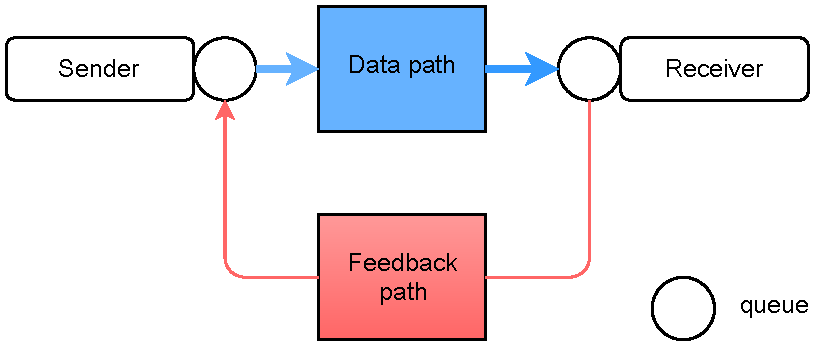
\includegraphics[width=0.8\textwidth]{./figures/simplefeedback.pdf}
      \caption[Multimedia feedback loop]{Multimedia feedback loop.}
	\label{fig:feedbackloop}
\end{figure}

%\subsection{Congestion control in real time media communication}
%
%Congestion control decisions in real time media communication are done periodically with the data retrieved from various sources, such as the feedback loop. This data helps the protocol to trigger special mechanisms that can modify the traffic shape of the peers that participate in the call. The factors that interact in this decision-making process are the metrics exposed in the following chapters.
%
%Different schemes can be given in congestion control mechanisms.
%
%Sender-driven rate adaptation is one of the methods to control the congestion of the link, his mechanism requires the sender to be aware of the status of the path. Different algorithms will then evaluate the congestion on the path and take decisions on how to send the media.
%
%Receiver-driven rate adaptation requires the receiver to study the status of the network and provide the best rate values back to the source of the data. Those values are then applied to the source of the traffic.
%
%Network-driven rate adaptation is the ability of the network to provide congestion information to the peers of a call about the capacity available and future variables. Once both peers have the new information of network rate, provided by some element of the network, they will be able to adjust to the new condition.
%
%There are two different types of congestion control: congestion avoidance and congestion mitigation.   
%
%Congestion avoidance is done before the link undergoes heavy congestion. Small congestion conditions can be detected by closely evaluating delay, jittering and different metrics. When doing congestion avoidance small changes occur in the sender to better adapt the rate.
%
%However, congestion mitigation is the action performed once the link is already handling heavy congestion. In this case, actions taken by the algorithms are drastic in order to mitigate congestion.
% 
% \begin{figure}[h]
%  \centering
%    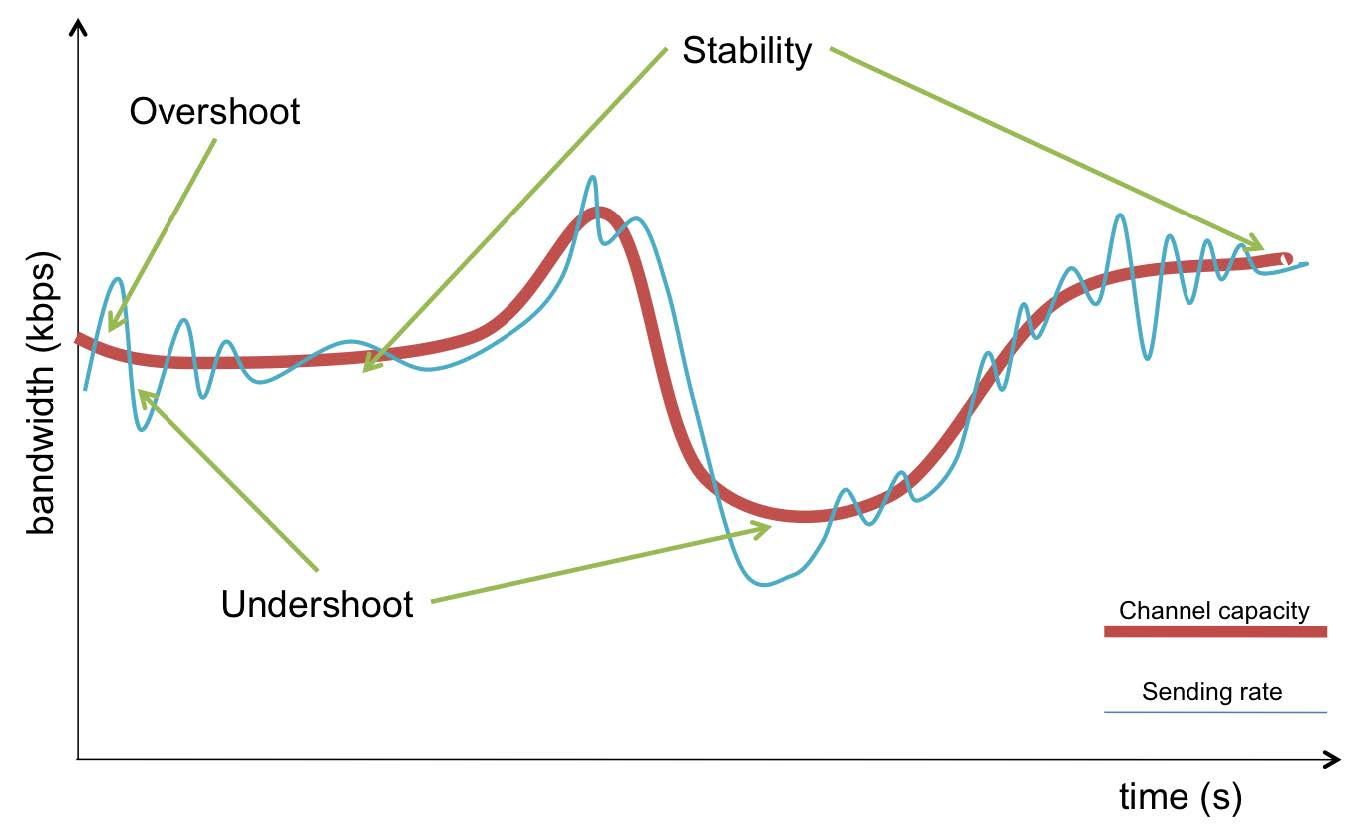
\includegraphics{./figures/rateadaptation.jpg}
%      \caption[Rate adaptation modes. Source~\cite{varunthesis}]{Rate adaptation modes. Source~\cite{varunthesis}.}
%	\label{fig:rateadaptation}
%\end{figure}
%
%When congestion is detected in the path, rate control algorithms operate in three different modes (Figure~\ref{fig:rateadaptation}): {\it overshoot}, {\it undershoot} and {\it stability}.
%
%Overshoot appears when the sending rate exceeds the capacity of the link, this mode of rate adaptation usually produces more congestion on the path and extra packet losses.
%
%Undershoot is the opposite behavior to Overshoot, it is given when heavy congestion appear on the link and packet losses occur. This produces a sudden conservative rate to avoid more losses and mitigate congestion.
%
%Stability is given when the capacity of the link is the same for a certain period of time, bandwidth rate may fluctuate but it will finally converge to the stable channel capacity on the path.
%
\subsection{Network metrics}

Metrics defined in this section are related to the status of the network, those metrics usually trigger the congestion control mechanisms in WebRTC changing the behavior of the stream according to the constraints on the link~\cite{rtpusageIETF}~\cite{alvestrandCongestion2012}. 

With real time applications, congestion affects protocol performance, if the media rate is lower than the available channel capacity there is no need for rate adaptation. However, losses and available capacity of the path can vary over time requiring adaptation from the sender side to match the new constraints. This adaptation is done by analyzing the receiver feedback packets sent to the sender using the simple feedback loop.

Three global factors are considered when analyzing network links: {\it loss}, {\it bandwidth} and {\it delay}.

\subsubsection{Losses}

Loss rate indicates packet losses during the transmission over the path. Usually packet losses affect directly the quality of a call. In WebRTC, packet loss is an indicator of the playback quality in the ongoing WebRTC transmission. In the case of huge packet loss in real-time media, the quality of the stream can be degraded producing artifacts on the playback.

When monitoring WebRTC calls we use packet loss as an indicator to adapt the media constraints. This indicator can be processed to be used along with the {\it GetUserMedia} constraints described in Section~\ref{sec:constraints} to adequate the media acquisition to the path condition. For example, an increase of packet loss could trigger some JavaScript mechanism that monitors the call quality and takes decisions based on the reported metrics. Those decisions may affect the video size and frames per second used to acquire the media. This allows a better adaptation for the ongoing session with the conditions on the path.

WebRTC uses RTCP packets for control and monitoring of the ongoing stream~\cite{rtcpIETF}. In RTCP losses are reported in the feedback message. Packet losses can also appear when being discarded by the protocol itself, this might happen due to heavy delay on the path.

Losses are calculated in a period of time, Equation~\ref{eq:PKTloss} calculates how much loss rate we have in a certain path. We subtract the packet loss given in a period and divide it between the difference of packets loss and received on that same period.  

\begin{equation}
	\frac{PKT_{loss}(T) - PKT_{loss}(T-1)}{PKT_{received}(T) - PKT_{received}(T-1) + PKT_{loss}(T) - PKT_{loss}(T-1)}
	\label{eq:PKTloss}
\end{equation}

Equation~\ref{eq:PKTloss} calculates the estimated packet loss we have on the link. This operation is done periodically by the statistical API described in Section~\ref{sec:constraints}.

\subsubsection{Round-Trip Time (RTT) and One-Way Delay (OWD)}

The delay on a path can be measured in two different forms. One-Way Delay (OWD) \nomenclature{OWD}{One-Way Delay} indicates the time it takes for a packet to move from one peer to the other peer, this time includes multiple delays that are produced along the link. OWD is calculated from the time taken to process the packet in both sides (building and encoding), the lower layer delay in the client (interface and intra-layering delay), queuing delay (from the multiple queues on the path) and propagation delay (speed of light). The sum of all those delays compose the total one-way delay.

\begin{equation}
	OWD = delay_{propagation} + delay_{queues} + delay_{serialization} + delay_{processing}	
	\label{eq:owd}
\end{equation}

In WebRTC applications, one of the most important delays that we have to measure is the processing delay. WebRTC applications usually run in a multiple layer structure. Running on top of the browser can affect the performance compared to other technologies that run directly over the OS. In the case of native mobile WebRTC applications, this delay is simnifically lower than in browser applications. 

%Delays in our case are symmetric as we are continuously sending and receiving media, low delay is important in order to reproduce the streams in the best quality possible and avoid uncomfortable communication. 

Round-Trip Time (RTT) \nomenclature{RTT}{Round-Trip Time} measurements are included in the standard RTCP specification, in order to calculate this metric, timestamp from sender and receiver is needed in the reports~\cite{rtcpIETF}. Sender Report (ST) timestamp is saved in the sender, meanwhile, the receiver returns the same timestamp in the Receiver Report (RR) that goes back to the origin. With those, we are able to calculate the RTT using the following Equation~\ref{eq:rtt}.

\begin{equation}
\label{eq:rtt}
\begin{split}
&RTT = TS_{RR} - TS_{SR} -T_{Delay}\\
 \quad &TS_{RR} \text{: Local timestamp at reception of last Receiver Report} \\
 \quad &TS_{SR}�\text{: Last Sender Report timestamp} \\
 \quad &T_{Delay} \text{: Receiver time period between SR reception and RR sending in the sender}
\end{split}
\end{equation}

We can calculate the RTT using the data given by the {\it Stats API} in WebRTC. This metric is important to be monitored as it indicates the time delay along the path and the playback quality on the endpoints.

Calculating OWD requires both machines clock to be accurately synchronized and can be complicated. Assuming that delay is symmetric we can define OWD as $\frac{RTT}{2}$. 

\subsubsection{Throughput}

Throughput is a key metric for measuring the performance of WebRTC applications. This indicator describes the capacity of the path taken by each {\it PeerConnection}. 

Furthermore, throughput can be divided into sending rate ($BR_S$), receiver rate ($BR_R$) and goodput ($GP$). From the technical point of view, sender rate is defined as the number of packets that are injected into the network by the sender. Receiver rate is the ratio at which packets arrive at the receiver. Goodput is the result of discarding all the lost packets from the total number along the path, only packets that have been received are counted, goodput is a good metric to measure performance. 

Typically, throughput is calculated by extracting the information from RTCP packets, in our case, we also rely on the Stats API included in WebRTC specification to calculate the rate. Taking into account the number of bytes received in the previous and actual period and the amount of time elapsed, we are able to calculate the throughput.

\begin{equation}
	\frac{\bigtriangleup Bytes_{received}}{\bigtriangleup Time_{host}}
	\label{eq:statsRate}
\end{equation}

The throughput defines the bandwidth usage for video/audio in each endpoint, we can use this value to get an overall quality status of the call. A sudden drop of the rate means that the bandwidth available for that {\it PeerConnection} has been drastically reduced, this introduces problems in the transmission, or in the worst case, loss of communication between peers.

\subsubsection{Inter-Arrival Time (IAT)}

Due to latency on the path, packets can arrive at different times, congestion causes the increase and decrease in Inter-Arrival Time (IAT) \nomenclature{IAT}{Inter-Arrival Time} between packets.

Congestion mechanisms in WebRTC use an adaptive filter that continuously updates the rate control of the sender side by using an estimation of network parameters based on the timing of the received frame. The actual mechanisms implement rate control by using IAT but other delay effects such as jitter are not captured by this model~\cite{alvestrandCongestion2012}. Jitter can be defined as the variation of IAT. The difference between when the packet is expected and when it is actually received is the jitter.

In WebRTC, IAT is given by the Equation~\ref{eq:iat},~\ref{eq:iat1} and~\ref{eq:iat2}~\cite{alvestrandCongestion2012}. This calculates the drift between the actual arrival time and the timestamp time of two packets (jitter), which should be approximately the same. 

\begin{equation}
\label{eq:iat}
\begin{split}
&d(i) = t(i) - t(i-1) - (T(i) - T(i-1))\\
 \quad &t \text{: arrival time } \\
 \quad &T \text{: timestamp time } \\
\end{split}
\end{equation}

Since the time $t_s$ to send a frame of size $L$ over a path with a capacity of $C$ is approximately:

\begin{equation}
\label{eq:iat1}
\begin{split}
&t_s = \frac{Size}{Capacity}\\
 \quad &Size \text{: Frame size } \\
 \quad &Capacity \text{: Capacity of the path } \\
\end{split}
\end{equation}

The final model for the IAT in WebRTC can defined as a function of serialization delay, queuing delay and network jitter.

\begin{equation}
\label{eq:iat2}
\begin{split}
d(i) = \frac{Size(i) - Size(i-1)}{Capacity} + w(i)
\end{split}
\end{equation}

Here, $w(i)$ is a sample $i$ from a stochastic process $W$ which is given in function of $C$, the current cross traffic $X(i)$ and the send bit rate $R(i)$. If the channel congestion is high $w(i)$ will increase, otherwise $w(i)$ it is going to decrease. Alternatively we can consider $w(i)$ equal to zero. IAT is usually calculated in the receiver and reported to the sender to enable sender-driven rate control.
%\subsubsection{Jitter}
%
%WebRTC streams are sent over the link in RTP format, those packets are generated sequentially. Due congestion on the path those packets may arrive in different order than in the source. Jitter is defined as the estimate of the statistical variance mean of the RTP packet inter-arrival time~\cite{rtcpIETF}.
%
%Inter-arrival time is a congestion indicator, Equation~\ref{eq:jitter} extracted from RTP RFC indicates how to calculate the approximate jitter~\cite{rtcpIETF}.
%
%\begin{equation}
%\label{eq:jitter}
%\begin{split}
%J_m &= J_{m-1} + \frac{D_{m-1} - J_{m-1}}{16}\\
% \quad m &= \text{received packets} \\
%\end{split}
%\end{equation}
%
%Jitter covers inter-arrival time information for the last 16 packets, in our case this will be useful as we will be using extended feedback profile (RTP/AVPF) for our media streams. In other scenarios jitter  be useful as it will only cover a part of the interval between two RTCP feedback messages.

\subsection{Host metrics}

Host metrics are measurements made locally by the host that affect the behavior of real time media communication. Those metrics do not need to be directly related to the network and can give information about the host performance when using WebRTC. They also provide information about timing and encoding for media in WebRTC sessions.

\subsubsection{Resources}

In WebRTC, we measure the local resource usage in the peers participating on a call, this metric is going to be very important for multiple peer topologies and resource demanding encoding.

CPU usage in WebRTC is critical. The web browser is the one in charge of the encoding and decoding process. This internal engine produces a huge load on the CPU. The amount of streams to handle will determine the status of the CPU. Having a normal load in the CPU helps WebRTC to perform better.

On the other side, RAM usage is also considered a constraint in any mobile or old device. The amount of RAM used in each WebRTC call relies in the encoding process and the network activity of the device. 

CPU/RAM usage is observed in order to calculate the stress on the host in WebRTC scenario. This information is crucial for the success of WebRTC in some topologies that demand large amount of resources.

\subsubsection{Setup time}

We also measure the setup time required for every topology, with this we can possibly determine an average setup time for WebRTC sessions. The setup time is calculated using local timestamps when building the {\it PeerConnection} object. WebRTC calls are divided into three processes, media acquisition, stream transfer over the network and remote video playback. The protocol itself is only based in the network transfer. However, the total time to establish the session is obtained once the playback of the remote stream starts. 

Once the media from the remote peer arrives, we can subtract both timestamps, start of the {\it PeerConnection} object and stream arrival, to check the elapsed time. This procedure is in the JavaScript layer.

\subsubsection{Call failure}

Call failure is an important metric that measures the software quality of a WebRTC application. Compared with the previous metrics, this indicator do not relate with topology issues. This also fully depend on NAT situations and we are going to calculate the average failed calls with STUN and TURN NAT technologies. This indicator can define the success ratio for establishing WebRTC calls.

%\subsubsection{Encoding and decoding}

%WebRTC statistical API also provides real time information about the encoding and decoding bit rate of the video codec. This metric usually varies depending on the congestion mechanisms that change in different path conditions, it is a good indicator for congestion and can give some hints about the way the encoding is done in WebRTC.

\subsection{Summary of metrics}

Performance metrics allow us to determine the behavior of the path. Those metrics are obtained by using the information provided in the RTCP messages and statistical APIs. We use them to evaluate each different scenarios and reach a conclusion about the performance of WebRTC.

Throughput, delay and loss are important metrics in WebRTC. They will assist congestion control mechanisms when adapting the sender rate for the media. Those metrics also define the quality of the media session and are important in order to improve the user experience when using WebRTC applications.

From the monitoring perspective, we care about characterizing the performance and congestion control algorithm of WebRTC. We study how those mechanisms behave and try to reach a consensus whether is a good alternative to use WebRTC or not. Lastly, some other metrics related to host help us to define which devices might be ready to hold WebRTC applications. 

%Based on the results we obtain for those indicators we can determine wether the congestion mechanisms are working as defined in the specs or should be improved for future versions of WebRTC.